% Ottawa U templates at http://www.uottawa.ca/brand/visual-identity/uottawa-template-spec-sheets
%fonts https://en.wikibooks.org/wiki/LaTeX/Fonts
% look at tcolorbox
%look at addtobeamertemplate to have margin
%550 h x 730 w

%header 30h font 7h w 282
%header 10h pagewidth


%footermargin 5
%bande 70 h x pagewidth
%font = 10h logo = 36h
%text at 25 du bas, logo at 21
%marg left = 24 marg right=16
%bas 15 h x pagewidth


\documentclass{beamer}
% \setbeameroption{show notes} %un-comment to see the notes
\usepackage[english]{babel}
\usepackage[utf8]{inputenc}
\usepackage{fancyvrb}
\usepackage[style=ieee]{biblatex}

%\usepackage[backend=bibtex, citesyle=numeric-comp, style=ieee, url=false]{biblatex}
\usepackage[backend=biber, style=ieee, url=false]{biblatex}
\addbibresource{References/refs.bib}
%\renewcommand{\footnotesize}{\tiny}


% *** MATH PACKAGES ***
%-----------------------------------------------
\usepackage{amssymb, amsfonts, mathtools}
\mathtoolsset{showonlyrefs=true}



% *** TABLE PACKAGES ***
%-----------------------------------------------
\usepackage{dcolumn, calc,booktabs}
\newcolumntype{d}[1]{D{.}{.}{#1}}

% *** FIGURES PACKAGES ***
%------------------------------------------------
\usepackage{color, tikz, graphicx, epstopdf, datatool, pgfplots}
\usetikzlibrary{positioning, calc, arrows, decorations, patterns, shapes}
\pgfplotsset{compat=1.9}


% *** EQUATIONS MACROS ***
%-----------------------------------------------
\newcommand{\vect}[1]{\mathbf{#1}}  
\newcommand{\mat}[1]{\mathbf{#1}}
\newcommand{\set}[1]{\mathcal{#1}}
\newcommand{\ins}{\in}
\newcommand{\matslamfullp}[3]{p(\vect{s}_{1:#1}, \set{M}|\vect{z}_{1:#2},\vect{u}_{1:#3}, \vect{s}_0)}
\newcommand{\matslamsampfac}[2]{p(\vect{s}_0) \prod\limits_{i=1}^{#1} p(\vect{s}_{i}| \vect{s}_{i-1}, \vect{u}_{i}) \prod\limits_{j=1}^{#2} p(\vect{z}_{j}| \vect{s}_{z_j}, \vect{l}_{z_j})}
\newcommand{\matslamsamplngaus}[3]{\sum\limits_{i=1}^#1  \|f_i(\vect{s}_{i-1}, \vect{u}_i) - \vect{s}_i\|^2_{\mat{\Sigma}_{u_i}} + \sum\limits_{i=1}^{#2}  \|h_i(\vect{s}_{z_i}, \vect{l}_{z_i}) - \vect{z}_i\|^2_{\mat{\Sigma}_{z_i}} - #3}


% *** HEADER AND SETUP ***
%------------------------------------------------
\mode<presentation>
{
  \usetheme{uottawa}
  \setbeamercovered{transparent}
  \setbeamertemplate{items}[circle]
}
\setbeamercolor{background canvas}{bg=white}

%\setbeamerfont*{uofooterfont}{size={\fontsize{\footerfont}{\footerfont}}}

%\useinnertheme{circles}
\newenvironment{selecaenv}{\only{\setbeamercolor{itemize item}{fg=garnet} \color{garnet}}}{}



% *** TITLE PAGE ***
%------------------------------------------------
\title{Text mining - Sentiment analysis \& Knowledge discovery\\\\
CSI 5387 Data Mining \& Concept Learning}
\author{Authors: Xiaoke Liu, Yan Zhang, and Diana Lucaci}
\date{\today}


%%%%%%%%%%%%%%%%%%%%%%%%%%%%%%%%%%%%%%%%%%%%%%%%%%%%%%%%%%%%%%%%
                        % Notes and resources
%%%%%%%%%%%%%%%%%%%%%%%%%%%%%%%%%%%%%%%%%%%%%%%%%%%%%%%%%%%%%%%%
% Intro and problem definition: https://monkeylearn.com/keyword-extraction/
%%%%%%%%%%%%%%%%%%%%%%%%%%%%%%%%%%%%%%%%%%%%%%%%%%%%%%%%%%%%%%%%

% *** SLIDES ***
%------------------------------------------------
\begin{document}

\maketitle

\setbeamertemplate{footline}[uottawatheme]


%%%%%%%%%%%%%%%%%%%%%%%%% New frame %%%%%%%%%%%%%%%%%%%%%%%%%

\begin{frame}
\frametitle{Table of Content}
\tableofcontents
\end{frame}


%%%%%%%%%%%%%%%%%%%%%%%%% New frame %%%%%%%%%%%%%%%%%%%%%%%%%

\section{Problem Definition}

%define the problem
\begin{frame}

\frametitle{Sentiment Analysis}
NLP main tasks:
\begin{itemize}
    \item \textbf{Classification}
    \item Unsupervised \textbf{keyword extraction} (important task for Text Mining, and Information retrieval)
\end{itemize}

\end{frame}


%%%%%%%%%%%%%%%%%%%%%%%%% New frame %%%%%%%%%%%%%%%%%%%%%%%%%  

\begin{frame}
\frametitle{Objectives}

\begin{enumerate}
    \item \textbf{Evaluate} the performance of different Machine Learning algorithms on the classification task
    \item \textbf{Compare} keyword extraction approaches in the context of sentiment classification
\end{enumerate}

\note{Brief introduction to State of the art (SLAM++ incremental update), go quickly over this}
\note[item]{note: Red and blue are not used to identify poses and landmarks}
\note[item]{left: only the bottom right of the matrix is recomputed}
\note[item]{left: more efficient but more fill-ins}
\note[item]{right: whole matrix recalculated}
\note[item]{right: increasing complexity, less fill-ins}
\note[item]{I investigated possible solutions to bridge the gap and dissociate ordering changes from full re-computation}

\end{frame}




%%%%%%%%%%%%%%%%%%%%%%%%% New frame %%%%%%%%%%%%%%%%%%%%%%%%%  

% \section{Previous work}
% % TODO brief overview of the task (in terms of datasets, applications, used baseline)
% \begin{frame}
% \frametitle{Sentiment Analysis}

% \end{frame}

% \begin{frame}
% \frametitle{Keyword extraction}

% \end{frame}

%%%%%%%%%%%%%%%%%%%%%%%%% New frame %%%%%%%%%%%%%%%%%%%%%%%%%  
\section{Data Set}
\begin{frame}{Sentiment Labelled Sentences}
\textbf{Sentiment Labelled Sentences Data Set}
From paper 'From Group to Individual Labels using Deep Features', Kotzias et. al,. KDD 2015'.
The data set contains attributes are text sentences, extracted from reviews of products, movies, and restaurants at different websites. Each records are labelled with positive or negative sentiment with following format:
\begin{table}[]
    \centering
    \begin{tabular}{c|c}
    \hline
         sentence&score  \\
         \hline
         ...& 1 (positive) \\
         ...& 0 (negative) \\
         \hline
    \end{tabular}
    \caption{Format}
    \label{tab:format}
\end{table}
\end{frame}
\note{Score is either 1 (for positive) or 0 (for negative)
The sentences come from three different websites/fields:

imdb.com
amazon.com
yelp.com

For each website, there exist 500 positive and 500 negative sentences. Those were selected randomly for larger datasets of reviews.
We attempted to select sentences that have a clearly positive or negative connotaton, the goal was for no neutral sentences to be selected.}

%%%%%%%%%%%%%%%%%%%%%%%%% Preprocessing %%%%%%%%%%%%%%%%%%%%%%%%%  
% \section{Preprocessing and Analysis}
% \begin{frame}
% \frametitle{data inspection}
% After loading each data set into data Frame, we can check the content of data. The data looks like following
% \begin{table}[]
%     \centering
%     \begin{tabular}{c|c|c}
%     \hline
%          &0&1  \\
%          \hline
%          0 & Wasted two hours. & 0\\
%          1 & Good case, Excellent value. & 1\\
%          2 & Great for the jawbone. & 1\\
%          3 & Would not go back. & 0\\
%          4 & The mic is great. & 1\\
%     \end{tabular}
%     \caption{Data Frame}
%     \label{tab:my_label}
% \end{table}
% \end{frame}
\begin{frame}{Data Visualization}
\centering
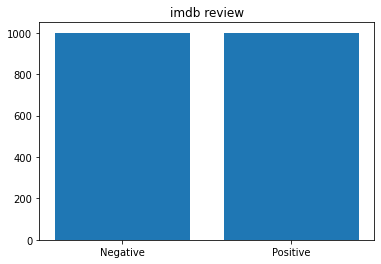
\includegraphics[width=.4\linewidth]{Figures/imdb_review.png}\quad%
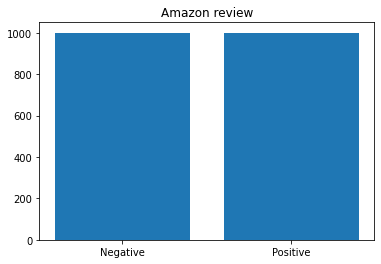
\includegraphics[width=.4\linewidth]{Figures/amazon_review.png}\quad%
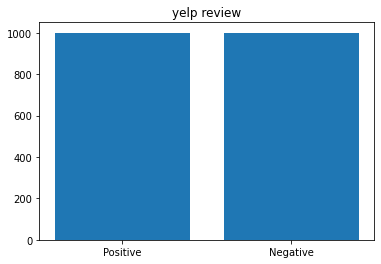
\includegraphics[width=.4\linewidth]{Figures/yelp_reivew.png}
\end{frame}
% \begin{frame}
% \frametitle{data inspection}
% After loading each data set into data Frame, we can check the content of data. The data looks like following
% \begin{table}[]
%     \centering
%     \begin{tabular}{c|c|c}
%     \hline
%          &0&1  \\
%          \hline
%          0 & Wasted two hours. & 0\\
%          1 & Good case, Excellent value. & 1\\
%          2 & Great for the jawbone. & 1\\
%          3 & Would not go back. & 0\\
%          4 & The mic is great. & 1\\
%     \end{tabular}
%     \caption{Data Frame}
%     \label{tab:my_label}
% \end{table}
% \end{frame}

% \begin{frame}{Vectorization}
%     \textbf {CountVectorizer}
%     \par Convert a collection of text documents to a matrix of token counts.
%     \par e.g. Corpus = [
%     \\   \setlength{\parindent}{48pt} ‘This is the first document.’,
% 	\\	‘This document is the second document.’,
% 	\\	‘And this is the third one.’,
% 	\\	‘Is this the first document?’,
%     ]
%     \\ \noindent Matrix = [0 1 1 1 0 0 1 0 1
%     \\ 0 1 0 1 0 2 1 0 1
%     \\ 1 0 0 0 1 0 1 1 0
%     \\ 0 1 1 1 0 0 1 0 1]
% \end{frame}

\begin{frame}{Vectorization}
    \textbf {TfidfVectorizer}
    \par Convert a collection of raw documents to a matrix of TF-IDF features.
    \par TF: Term Frequency
    \begin{center}
    \\ $TF(t)=\frac{Number\, of\, items\, term\, t\, appears\, in\, a\, document}{Total\, number\, of\, terms\, in\, the\, document}$
    \end{center}
    \par IDF: Inverse Document Frequency
    \begin{center}
    \\ $IDF(t)=\log_{e}\frac{Total\, number\, of\, documents}{Number\, of\, documents\, with\, term\, t\, in\, it\,}$
    \end{center}
\end{frame}

% \begin{frame}{text manipulation}
% we further remove the stop words and any special characters and brackets from the data set. Moreover, we reduce each word by simple stemming technique and we finally get the data set looks like:
% \begin{table}[]
%     \centering
%     \begin{tabular}{c|c}
%   review&sentiment\\
%   \hline
%   way plug US unless go convert&0\\
%   good case excel valu&1\\
%   great jawbon&1\\
%   tie charger convers last 45 minutesmajor problem&0\\
%   mic great&1\\
%     \end{tabular}
%     \caption{Reduced data frame}
%     \label{tab:reduce}
% \end{table}
% \end{frame}

%%%%%%%%%%%%%%%%%%%% Model  %%%%%%%%%%%%%%%%%%%%%%%%%%%
\section{Model Construction}

\begin{frame}{Model Selection}
    To be able to predict new entries, we utilized several methods to build models and fit the given data set.
    In model construction step, we tried the following options
    \begin{enumerate}
        \item Na\"ive Bayes
        \item SVM
        \item MLP
    \end{enumerate}
\end{frame}
\begin{frame}{}
\begin{enumerate}
    \item \textbf{Naive Bayes}
    $$P(Class|Sentence)=\frac{P(Sentence|Class)P(Class)}{P(Sentence)}$$
    \item \textbf{SVM}
    
    searches for the linear optimal separating hyperplance that best separate different classes.
    \item \textbf{MLP}
    
    classify classes based on computational network simulate perceptron
    
\end{enumerate}
\end{frame}

\begin{frame}[fragile]
\begin{columns}
\begin{column}{0.5\textwidth}
\begin{figure}
    \centering
    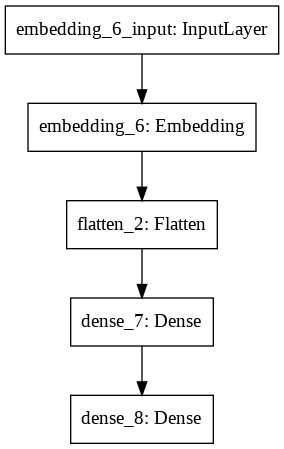
\includegraphics[width=0.6\linewidth]{Figures/mlp_structure.png}
    \caption{MLP structure}
    \label{fig:mlp_struc}
\end{figure}
\end{column}
\begin{column}{0.5\textwidth}
This simple NN has the structure
\begin{table}[fontsize=\small]
    \centering
    \begin{tabular}{c|c}
    \hline
     Layer (type)&Output Shape\\
     \hline\hline
     Embedding&(None, 74, 32)\\
     \hline
     Flatten&(None, 2368)\\
     \hline
     Dense&(None, 250)\\
     \hline
     Dense&(None, 1)\\
     \hline\hline
\end{tabular}
\end{table}
\end{column}
\end{columns}
\end{frame}

\section{Evaluation}
\subsection{Classification}
\begin{frame}{Result}
    \begin{table}[]
        \centering
        \begin{tabular}{|c|c|c|c|c|c|}
        \hline
        &Accuracy&Sentivity&Specificity&Percision&AUC\\
        \hline
        Na\"ive Bayes&82.17\%&84\%&81\%&81\%&89.89\%\\
        \hline
        SVM&83.67\%&85\%&83\%&83\%&91.19\%\\
        \hline
        MLP&77.33\%&76\%&79\%&80\%&85\%\\
        \hline
        \end{tabular}
        \caption{Evaluation}
        \label{tab:my_label}
    \end{table}
\end{frame}

\begin{frame}{ROC curve}
\centering
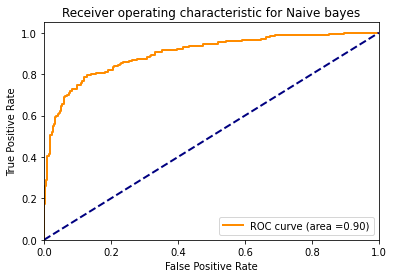
\includegraphics[width=.4\linewidth]{Figures/nb_roc.png}\quad%
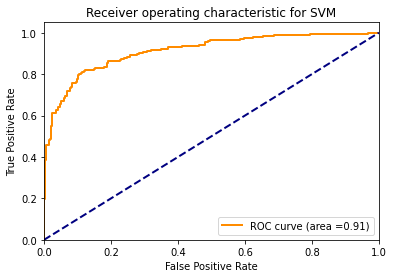
\includegraphics[width=.4\linewidth]{Figures/svm_roc.png}\quad%
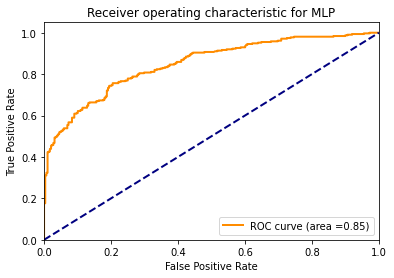
\includegraphics[width=.4\linewidth]{Figures/mlp_roc.png}
\end{frame}
%%%%%%%%%%%%%%%%%%%%%%%%% New frame %%%%%%%%%%%%%%%%%%%%%%%%%

%Datasets used
% \section{Results}

% \begin{frame}
% \frametitle{Dataset - Motivation}

% \begin{itemize}
% \item Accessible interpretation of the results, in the context of sentiment analysis
% \end{itemize}
% \end{frame}



\subsection{Keyword and Keyphrase extraction}
%%%%%%%%%%%%%%%%%%%%%%%%% New frame %%%%%%%%%%%%%%%%%%%%%%%%%  
\begin{frame}
\frametitle{Task and evaluation metrics}

\begin{columns}[T]

\begin{column}{0.5\textwidth}
\textbf{Classification}
\begin{itemize}
\item Accuracy
\item Precision
\item Recall
\item F1
\item AUC
\end{itemize}

\end{column}
\vrule{}
\begin{column}{0.5\textwidth}
\textbf{Keyword-extraction}
\\ - unsupervised task, analyzing the generated phrases/words through:
% Note: Summarization, information retrieval (search engines)
\begin{itemize}
\item Quantitative analysis
\item Qualitative analysis
\end{itemize}

\end{column}
\end{columns}
\end{frame}

\begin{frame}
\frametitle{Quantitative analysis}
     \begin{itemize}
        \item frequency in each corpora
        \item polarity
        \item the impact on the classification task
    \end{itemize}   
\end{frame}
\begin{frame}{Qualitative analysis}
        \begin{itemize}
        \item statistical metrics
        \item word cloud
        \item visualization techniques
        \item application-grounded evaluation
    \end{itemize}
\end{frame}

%%%%%%%%%%%%%%%%%%%%%%%%% New frame %%%%%%%%%%%%%%%%%%%%%%%%%  


\begin{frame}
\frametitle{Methods}

\begin{itemize}
    \item Statistical methods
    \begin{itemize}
        \item TF-IDF
        \item RAKE
        \item YAKE
    \end{itemize}
    \item Graph-based methods
    \begin{itemize}
        \item TextRank
    \end{itemize}
\end{itemize}

\end{frame}



\begin{frame}
\footnotesize
\frametitle{Quantitative - classification task}
    \begin{table}[]
        \centering
        \begin{tabular}{|c|c|c|c|c|c|c|}
        \hline
        Model& Dictionary&Accuracy& Precision & Recall & F1\\
        \hline
        Vanilla - LSTM& &82.68 & 0.8449 & 0.7938 & 0.8135
        \\\hline
        LSTM+MLP\_gen&TF-IDF& 79.44 & 0.8619 & 0.6888 & 0.7612 & 0.7828\\
        &RAKE\_corpus&82.51 & 0.8253 & 0.8158 & 0.8169 \\
        &RAKE\_instance&82.68 & 0.8276 & \textbf{0.8168} &\textbf{ 0.8186} \\
        &YAKE & \textbf{83.00 }& 0.8501 & 0.7919 & 0.8153\\
        & TextRank &82.84 & \textbf{0.8629} & 0.7788 & 0.8139\\
        \hline
        \end{tabular}
        \caption{Keyword extraction evaluation}
        \label{tab:ke_eval}
    \end{table}
\end{frame}

\begin{frame}{Qualitative - metrics}
    \begin{table}[]
        \centering
        \begin{tabular}{|p{1.5cm}|p{2cm}|p{2cm}|p{2cm}|p{1cm}|}
        \hline
        Dictionary type& Avg words / keyphrase (dataset)& Avg words / keyphrase (pos) &Avg words / keyphrase (neg) & Overlap count\\\hline
        
        TF-IDF &1&1&1&21\\ \hline
        RAKE (corpus)&3.61&3.74&3.48&0\\ \hline
        RAKE (instance)&4.14&4.3&3.98&0\\ \hline
        YAKE&1.85&1.89&1.82&23\\ \hline
        TextRank&1.13&1.15&1.11&5\\ \hline
        
        
        \end{tabular}
        \caption{Keyphrase analysis for dictionaries of 300 entries}
        \label{tab:ke_eval}
    \end{table}

\end{frame}
\begin{frame}{Qualitative}
\begin{figure}
\centering
\begin{minipage}{.5\textwidth}
  \centering
  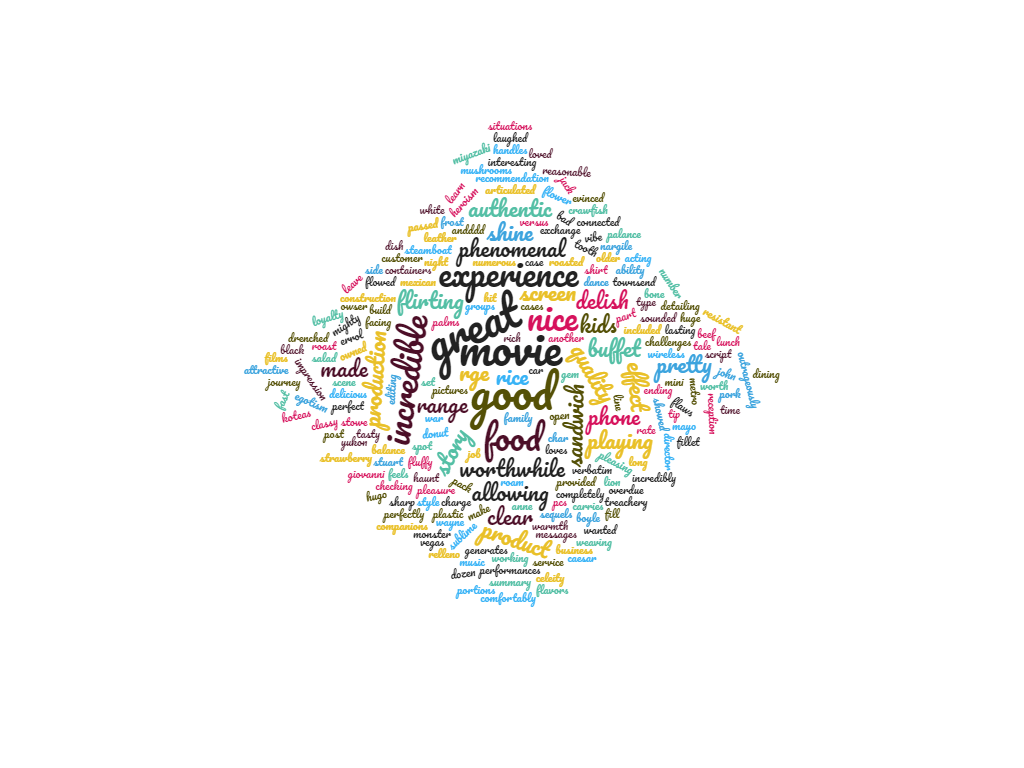
\includegraphics[width=1.35\linewidth]{Figures/yake_pos.png}
  \captionof{YAKE - positive}
  \label{fig:test1}
\end{minipage}%
\begin{minipage}{.5\textwidth}
  \centering
  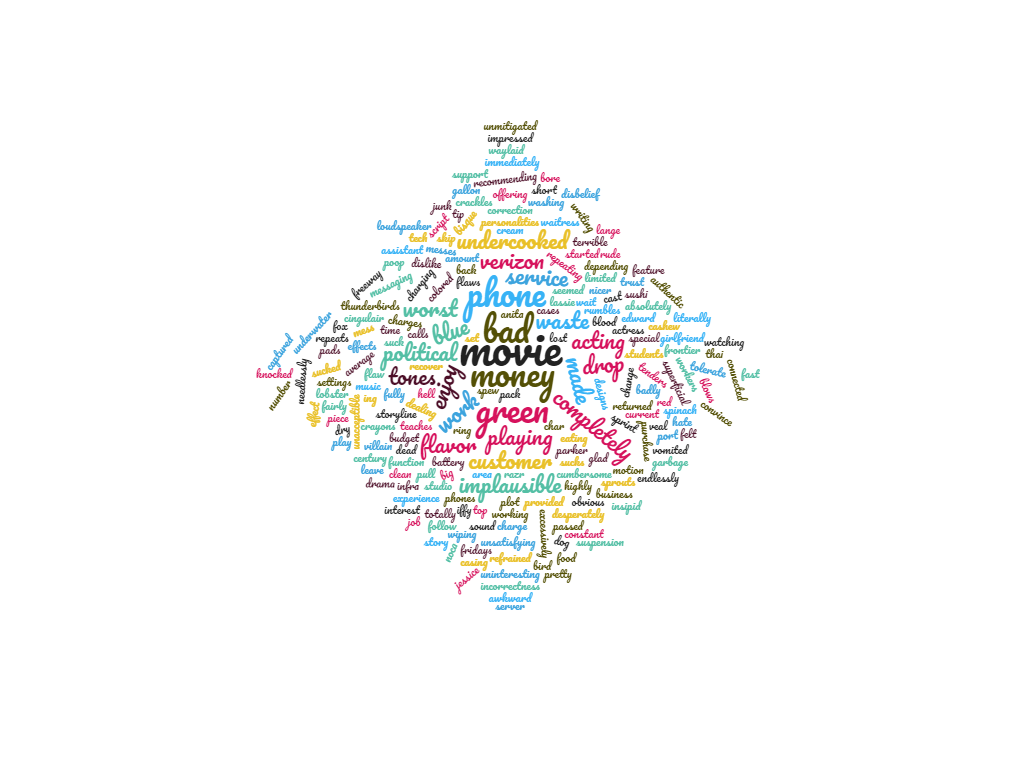
\includegraphics[width=1.35\linewidth]{Figures/yake_neg.png}
  \captionof{YAKE - negative}
  \label{fig:test2}
\end{minipage}
\end{figure}
\end{frame}
%%%%%%%%%%%%%%%%%%%%%%%%% New frame %%%%%%%%%%%%%%%%%%%%%%%%%

\section{Contributions}
\frametitle{\phantom{ }}
\begin{frame}{Summary}

\begin{itemize}
\item Comparative analysis of ML algorithms on the classification task
\item Literature review on keyword extraction algorithms
\item Evaluation methods for the keyword extraction tasks
\item Preliminary results and analysis
	
\end{itemize}

\end{frame}



%%%%%%%%%%%%%%%%%%%%%%%%% New frame %%%%%%%%%%%%%%%%%%%%%%%%%  

\section{Future Work}

%future work
\begin{frame}
\frametitle{\phantom{ }}

Possible avenues of extending the projects include
\begin{itemize}
    \item Apply the methodology on different domains, text data sets, and tasks
    \item Extending the battery of experiments
\end{itemize}

\end{frame}




%%%%%%%%%%%%%%%%%%%%%%%%% New frame %%%%%%%%%%%%%%%%%%%%%%%%%

\section{Questions and Comments}

\begin{frame}[c]

\frametitle{\phantom{ }}

\centering
\Huge
Thank you.

\end{frame}

\end{document}





%%% Local Variables:
%%% mode: latex
%%% TeX-master: t
%%% End:
